% XeLaTeX can use any Mac OS X font. See the setromanfont command below.
% Input to XeLaTeX is full Unicode, so Unicode characters can be typed directly into the source.

% The next lines tell TeXShop to typeset with xelatex, and to open and save the source with Unicode encoding.

%!TEX TS-program = xelatex
%!TEX encoding = UTF-8 Unicode

\documentclass[11pt,a4paper,left=15mm,right=15mm,top=20mm,bottom=20mm]{article}
\usepackage{geometry}                % See geometry.pdf to learn the layout options. There are lots.
\usepackage[hangul]{kotex}
\usepackage{indentfirst}
\geometry{letterpaper}                   % ... or a4paper or a5paper or ... 
%\geometry{landscape}                % Activate for for rotated page geometry
%\usepackage[parfill]{parskip}    % Activate to begin paragraphs with an empty line rather than an indent
\usepackage{graphicx}
\DeclareGraphicsExtensions{.pdf,.png,.jpg,.jpeg}
\usepackage{amssymb}

\usepackage{listings}

% uml package
\usepackage{tikz}

% Will Robertson's fontspec.sty can be used to simplify font choices.
% To experiment, open /Applications/Font Book to examine the fonts provided on Mac OS X,
% and change "Hoefler Text" to any of these choices.

\usepackage{fontspec,xltxtra,xunicode}
\defaultfontfeatures{Mapping=tex-text}
\setmainhangulfont{Sarasa Mono K Nerd Font Complete}
\setromanfont[Mapping=tex-text]{Sarasa Mono K Nerd Font Complete}
\setsansfont[Scale=MatchLowercase,Mapping=tex-text]{Sarasa Mono K Nerd Font Complete}
\setmonofont[Scale=MatchLowercase]{D2Coding}

\title{Alcor}
\author{yongmin}
%\date{}                                           % Activate to display a given date or no date

\begin{document}
\maketitle

\tableofcontents
\listoffigures

\newpage

\section{과제 목표}

이 과제는 클라이언트로 하여금 신뢰할 수 있는 투표 시스템을 만드는 것이 목표이다. 그렇게 하기 위해 서버가 함부로 데이터를 조작할 수 없는 환경을 만들고 모든 과정 사이에 서버와 클라이언트만 정보를 안전하게 주고 받고 열람할 수 있어야한다. 또한 클라이언트는 서버에서 저장하고 결과를 산출할 때 사용한 데이터를 받아서 테스트하여 부정을 검출할 수 있어야한다. 또한 서버를 필요에 따라 확장할 수 있게 하여 필요한 기능을 추가하거나 예상 되는 트래픽을 비교적 쉽게 처리할 수 있어야한다.

\section{과제 구성}

위 목표를 달성하기 위해 해당 과제는 크게 4개 영역으로 구성된다.

    \subsection{서버}

        \subsubsection{후보 추가, 수정 및 삭제}

        \begin{figure}[h]
            \begin{center}
                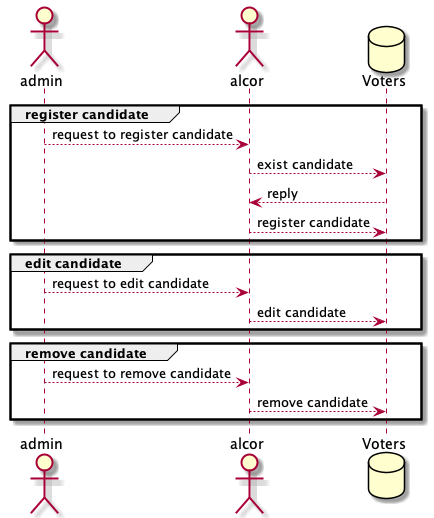
\includegraphics[width=10cm]{candidate-reg}
                \caption{후보 시퀸스 다이어그램}
            \end{center}
        \end{figure}

        서버는 관리자 앱을 통하여 후보를 추가할 수 있다. 관리자 앱은 서버에 후보 정보를 보내고 서버는 데이터베이스에 기록하고 그 결과를 반환한다. 주요 에러는 이름이 중복되어 투표 시 유권자가 식별할 수 없을 때 발생한다. 

        또한 관리자 앱은 후보의 정보를 수정하여 전송함으로 후보를 삭제하고 재등록, 즉 수정할 수 있다.

        삭제 또한 관리자 앱에서 서버에 요청하면 서버는 존재하는 후보인지 파악하여 삭제를 수행한 후 결과를 반환한다.

        \subsubsection{유권자 등록}

        \begin{figure}[h]
            \begin{center}
                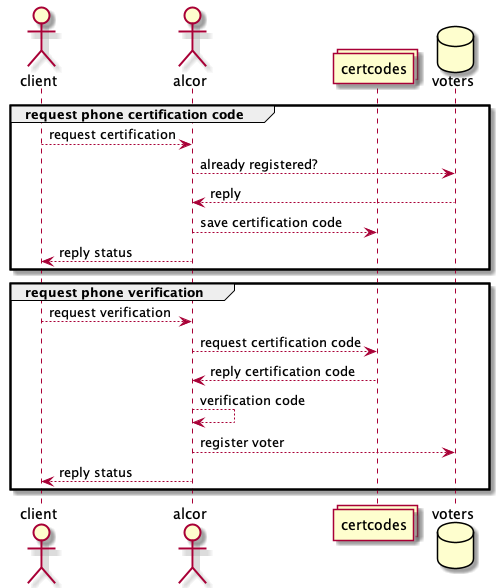
\includegraphics[width=10cm]{client-register}
                \caption{유권자 등록 시퀸스 다이어그램}
            \end{center}
        \end{figure}

        

        \subsubsection{투표}

        \subsubsection{설문조사}

        \subsubsection{투표 결과 조회}

        \subsubsection{설문조사 조회}

    \subsection{클라이언트}

        \subsubsection{유권자 등록}

        \subsubsection{투표}

        \subsubsection{설문조사 작성}

    \subsection{관리자}

        \subsubsection{후보 등록}

        \subsubsection{후보 수정 및 삭제}

    \subsection{옵저버}

        \subsubsection{결과 조회}

        \subsubsection{데이터 검증}

        \subsubsection{설문조사 통계 조회}

\section{개발 환경 및 도구}

    \subsection{서버}

        \subsubsection{개발 환경}

            macOS 10.15 이상, windows 10 이상

        \subsubsection{도구}

            visual studio code와 golang 1.17 이상, docker 필요

        \subsubsection{대상 환경}

            docker가 설치된 모든 리눅스 배포판

    \subsection{클라이언트}

        \subsubsection{개발 환경}

            macOS 10.15 이상, windows 10 이상

        \subsubsection{도구}

            visual studio code와 android studio를 IDE로 사용하고 dart 2.0 이상, flutter 2.0 이상

        \subsubsection{대상 환경}

            linux, windows, macOS, android

    \subsection{관리자}

        \subsubsection{개발 환경}

            macOS 10.15 이상, windows 10 이상

        \subsubsection{도구}

            visual studio code와 android studio를 IDE로 사용하고 dart 2.0 이상, flutter 2.0 이상

        \subsubsection{대상 환경}

            linux, windows, macOS, android

    \subsection{옵저버}

        \subsubsection{개발 환경}

            macOS 10.15 이상, windows 10 이상

        \subsubsection{도구}

            visual studio code와 golang 1.17 이상, python 3.7 이상, docker 필요

        \subsubsection{대상 환경}

            docker가 설치된 모든 OS

\section{부록}

\end{document}